\chapter{Communication between devices}
%Key words: Master slave, block diagram, pull up res, cmd controlled,  
%pi pull up = $1.8k\Omega$
Communication between the various device in the robot is a vital issue. Without proper communications the robot will not be able to function after the intention. In this project the communication protocol has been chosen to be the I$^2$C protocol because is it more flexible then for example the SPI protocol.    
\section{I$^2$C}
The I$^2$C (Inter-Integrated Circuit) protocol is a very used communication method in electronic devices. It is a two way multi-master communications protocol where there is one interchangeable master and up to 112 slave devises. The master device sets the clock (SCL) and sends out a data stream on the data line (SDA) starting with a byte containing a 7 bit address for the decided slave device, and a read/write bit the determines what action the master device wants do execute. After the address byte follows data transfered one byte at the time until there is no more data to transfer. A pull up resistor is added to each of the to lines to ensure that the lines a pulled high when the bus is not i use and between pulse during transmitting.

\begin{figure}[!h]
	\centering
	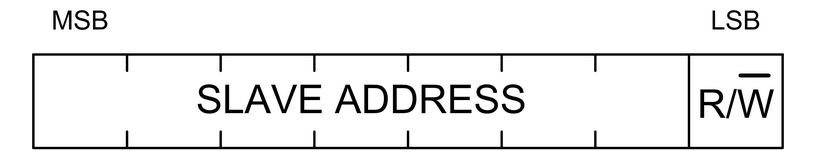
\includegraphics[width=0.4\textwidth]{commnuication_i2c_address.png}
	\caption{Address byte used by the I$^2$C protocol}
	\label{fig:communication_I2C_address}
\end{figure}


\begin{figure}[!h]
	\centering
	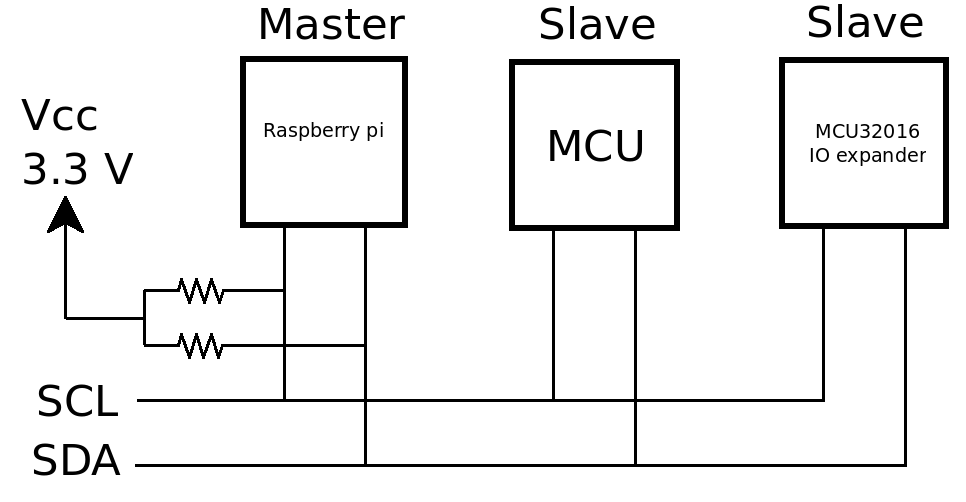
\includegraphics[width=0.5\textwidth]{communication_i2c_diagram.png}
	\caption{Block diagram of the I$^2$C bus}
	\label{fig:communication_I2C_diagram}
\end{figure}
\newpage
\section{Implementation}
In this project the Raspberry pi is the I$^2$C master because it is within this devise all the processing in produced. The Raspberry pi is running the I$^2$C bus at 100kHz and is equipped with two 1.8k$\Omega$ pull up resistors.\\ To make the communication procedure easier, a command system has been implemented in all the devices attached to the I$^2$C bus (not the IO expander because this device it a static I$^2$C device). The system makes the first data byte in the data stream to a command(CMD) and this command then calls different functions that deals with the rest of the data in the stream.   



\subsection{I$^2$C Commands}
The I$^2$C commands are:

\begin{itemize}
	\begin{item}
		\textbf{ CMD 0x05}: cmd set led\\ The raspberry pi writes one byte that controls the three LEDs on the motor controller board.
	\end{item}

	\begin{item}
		\textbf{ CMD 0x10}: cmd get speed\\ read two bytes of data that contains the speed for each motor calculated in the MCU.
	\end{item}
	
	\begin{item}
		\textbf{ CMD 0x20}: cmd set speed \\ Raspberry pi Writes two bytes to set the motor speed by changing the PWM value.
	\end{item}	
	
	\begin{item}
		\textbf{ CMD 0x30}: cmd set dir\\ Raspberry pi writes two byte that sets the detection on the motors by changing the four direction bits in the MCU.
	\end{item}

	\begin{item}
		\textbf{CMD 0x50}: cmd set state\\ Raspberry pi writes one bite that changes the states in the MCU between Speed, Position and Straight. 
	\end{item}
	
	\begin{item}
		\textbf{ CMD 0x60}: \\ spørg Jacob ??
	\end{item}
	
	\begin{item}
		\textbf{CMD 0x70}:  cmd precision stop\\ Sets the position and target variables to zero.
	\end{item}

	\begin{item}
		\textbf{CMD 0x80 }: cmd get dist\\ Raspberry pi reads three bytes that contains the distance from the three IR distance sensors.
	\end{item}
	
	\begin{item}
		\textbf{CMD 0x90 }: cmd enable dist\\ Enables the three ADC channels in the MCU that converts the IR distance sensors.
	\end{item}			

	\begin{item}
		\textbf{ CMD 0xA0}: cmd is stable. \\ Spørg Jacob ??
	\end{item}		

\end{itemize}